\chapter{Methods}
\label{chap:methods}

%--------------------------------------------------------------------------------------------------------------------------------------------
\section{Methodology}

This thesis uses a methodology for machine learning experiment design \parencite{fernandez-lozanoMethodologyDesignExperiments2016}. The methodology consists of a workflow with the following steps: Dataset, Data Preprocessing, Model Learning and Best Model Selection. The main focus of the thesis is on Model Learning and Best Model Selection with an emphasis of using system performance metrics. Advanced preprocessing techniques or achieving state of the art model performance are out of the scope of this thesis.

\improvement{TODO Vertailukriteeristö: tapana ohjelmistopuolella + tapana koneoppimispuolella}

This master's thesis asks the following research questions:
\begin{itemize}
    \item \emph{RQ1}: How does system performance change over time during model training?
    \item \emph{RQ2}: How do changes in hyperparameters affect system performance during model training?
    \item \emph{RQ3}: How does early stopping on system performance criteria affect computational budgets during model training?
          
\end{itemize}

\section{Experimental setup}

\subsection{Software and Hardware}

Experiments were performed using Ray Tune (2.7.1) \parencite{liawTuneResearchPlatform2018}. MLFlow (2.7.1) \parencite{chenDevelopmentsMLflowSystem2020} was used for recording metrics and tracking experiments. Scikit-learn (1.3.2) \parencite{pedregosaScikitlearnMachineLearning2011} for training, collecting machine learning performance metrics and evaluating machine learning models. Psutil \parencite{rodolaGiampaoloPsutil2023} was used for collecting system performance metrics from the operating system. Hardware used to perform the experiments consisted of Intel Core i7-9700 @ 3.00GHz CPU and Nvidia 3060 GPU.

\subsection{Datasets}


OpenML \parencite{vanschorenOpenMLNetworkedScience2014} was a source of benchmarking datasets for both classification \parencite{bischlOpenMLBenchmarkingSuites2017} and regression \parencite{fischerOpenMLCTR23CuratedTabular2023} tasks. In total two classification task and two regression task datasets summarized in table~\ref{table:datasets} were chosen to keep the amount of computation reasonable.

The \emph{mnist\_784} dataset consisted of $70000$ images of handwritten digits with each feature representing a pixel with the task to classify which digit the image represents. The \emph{diabetes} dataset consisted of $785$ measurements of female patients with the task to classify whether the patient tests positive for diabetes. The \emph{wave\_energy} dataset consisted of $72000$ different positions for 16 buoys with the regression task to predict the total amount of energy produced. The $16$ wave energy converter features were dropped as the target variable is total energy. The \emph{red\_wine} dataset consisted of $1599$ measurements of red wine samples with the regression task of predicting the quality of the wine.

\begin{table}[h]
    \centering
    \begin{tabular}{lllll}
        \toprule
        Dataset      & Type    & Task           & Instances & Features \\
        \midrule
        mnist\_784   & image   & classification & 70000     & 785      \\
        diabetes     & tabular & classification & 768       & 9        \\
        wave\_energy & tabular & regression     & 72000     & 33       \\
        red\_wine    & tabular & regression     & 1599      & 12       \\
        \bottomrule
    \end{tabular}
    \caption{Summary of the datasets used.}
    \label{table:datasets}
\end{table}

\subsection{Algorithms}

Algorithms were chosen to support training in batches without being computationally heavy. Linear regression, logistic regression and support vector machine (SVM) are based on stochastic gradient descent (SGD) implementation found in Scikit-learn \parencite{pedregosaScikitlearnMachineLearning2011}. Algorithms and hyperparameters are summarized in Table~\ref{table:algorithms}. Model training, evaluation and hyperparameter optimization was performed in parallel with each worker process using one CPU core each.

Hyperparameters such as batch size, learning rate and regularization alpha are selected using grid search with the search space determined with preliminary experiments so that the optimal solution is not too close to the boundaries. Batch size search space was $2^i$ for all $i$ from $1$ until $2^i$ was equal to the number of samples in the dataset. Learning rate search space was $10^i$ for all $i$ between $-1$ and $-4$ \improvement{Parempi tapa esittää, että batch size oli 2. potenssi välillä 2-n ja learning rate oli 10. potenssi välillä 0.1 - 0.0001}.

\improvement{TODO: Add early stopping}


\begin{table}[h]
    \centering
    \begin{tabular}{lll}
        \toprule
        Algorithm              & Loss    & Hyperparameters                  \\
        \midrule
        Linear regression      & squared & batch size, learning rate, alpha \\
        Logistic regression    & log     & batch size, learning rate, alpha \\
        Support Vector Machine & hinge   & batch size, learning rate, alpha \\
        \bottomrule
    \end{tabular}
    \caption{Summary of the algorithms}
    \label{table:algorithms}
\end{table}

\subsection{Metrics and evaluation}
Metrics to be evaluated can be divided into machine learning metrics and system performance metrics and are summarized in Table~\ref{table:metrics}. Machine learning metrics consisted of training loss, validation loss, accuracy for classification and root mean square error for regression respectively. System compute performance was measured through mean training step time and cpu utilization percentage. System memory performance was measured through memory use of the process and computational budget was measured as elapsed wall-time required for training the model. Training loss was computed with each training step and the rest of the metrics were computed every $100$ training steps. Machine learning metrics were computed using scikit-learn \parencite{pedregosaScikitlearnMachineLearning2011} and system performance metrics were collected from the operating system using psutil \parencite{rodolaGiampaoloPsutil2023}.

\begin{table}[h]
    \centering
    \begin{tabular}{llll}
        \toprule
        Metric                  & Type               \\
        \midrule
        training loss           & machine learning   \\
        validation loss         & machine learning   \\
        accuracy                & machine learning   \\
        root mean square error  & machine learning   \\
        mean training step time & system performance \\
        total training time     & system performance \\
        cpu utilization (\%)    & system performance \\
        memory (MB)             & system performance \\
        \bottomrule
    \end{tabular}
    \caption{Summary of the metrics}
    \label{table:metrics}
\end{table}

In accordance with Ray documentation \parencite{therayteamMemoryManagementRay} to avoid double counting memory used by the object store the memory usage of the worker was computed in the following way:

\[ \text{memory} = \text{resident set size (RSS)} - \text{shared memory usage (SHR)} \]

Machine learning models were validated by splitting the dataset into a $70\%$ training set and a $30\%$ test set. To make sure that measurements are not sensitive to chosen data ten-fold cross validation using the training set was performed when tuning hyperparameters.


\improvement{TODO rank-based analysis using Friedman and Nemenyi post-hoc test \parencite{fischerOpenMLCTR23CuratedTabular2023}, bonferroni correction}

\subsection{Machine learning workflow}

The following workflow was performed for each dataset:

\begin{enumerate}
    \item Downloading the dataset in OpenML Dataset format
    \item Transforming an OpenML Dataset to a Ray Dataset
    \item Splitting the data into training and test datasets
    \item Splitting the training data into 10-folds
    \item Normalizing the training data for each fold and applying the transformation to the test dataset
    \item Tuning each hyperparameter for each fold
    \item Training the model
    \item Early stopping if criteria are met
\end{enumerate}

\begin{figure}[h]
    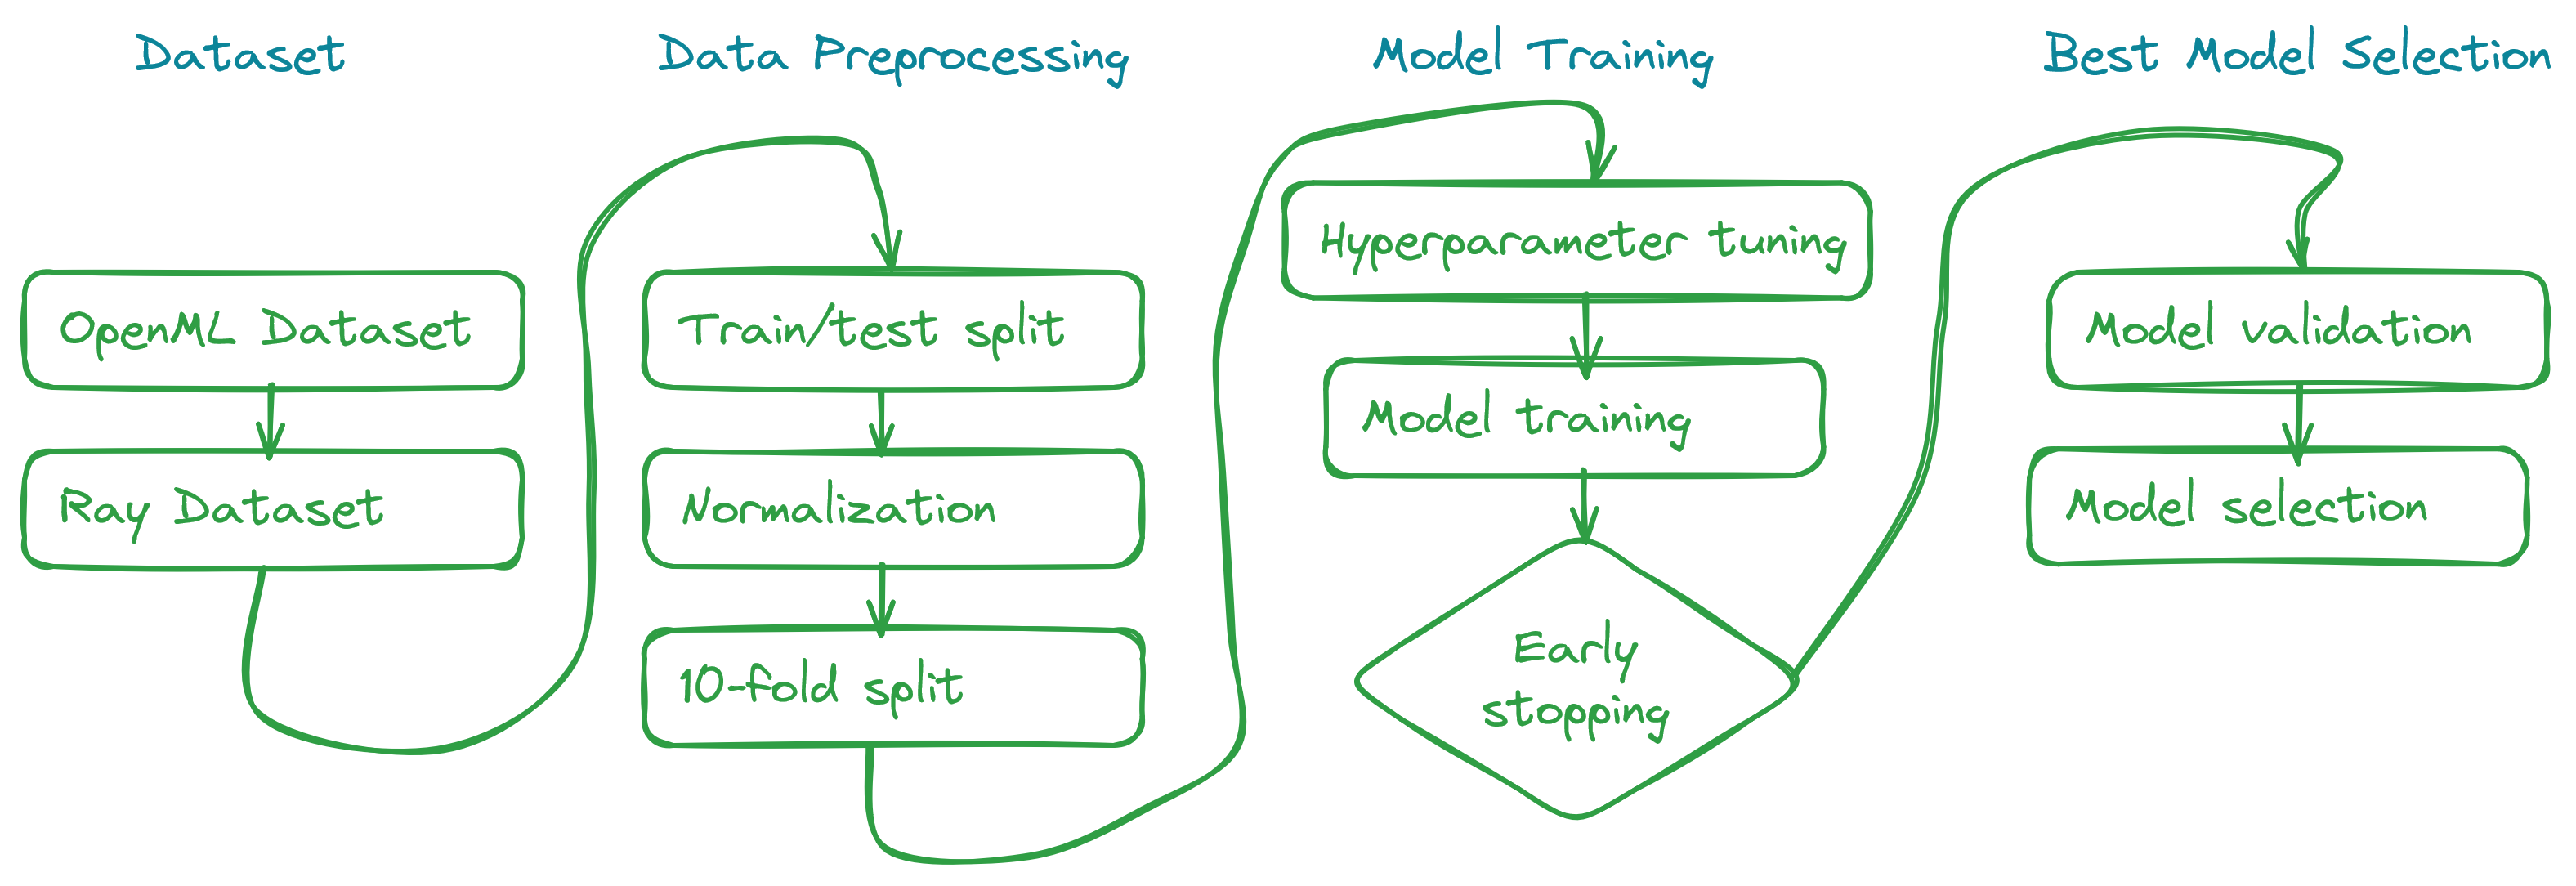
\includegraphics[width=12cm]{assets/ml_workflow1.png}
    \caption{TODO placeholder image: ML workflow}
    \label{figure:mlworkflow}
\end{figure}

\section{Experiments and Results}

First set of experiments were performed to determine whether system performance is constant during model training. Second set of experiments were performed to determine how changes in the hyperparameters affect system performance metrics. For each metric the average of all the runs was visualized and inspected for clear patterns with the focus on system performance metrics. Final set of experiments were performed to determine how setting a system performance criterion affects the computational budget can reduce the computational budget.




\subsection{Changes in system performance during model training}


The behavior of machine learning metrics was as expected with both the training loss and the validation loss decreased during training with the validation loss eventually plateaued. Accuracy had high variability and did not clearly increase or decrease during model training. An example of ML metrics with SVM trained on MNIST dataset ~\ref{figure:mlmetrics}. 

\begin{figure}[h]
    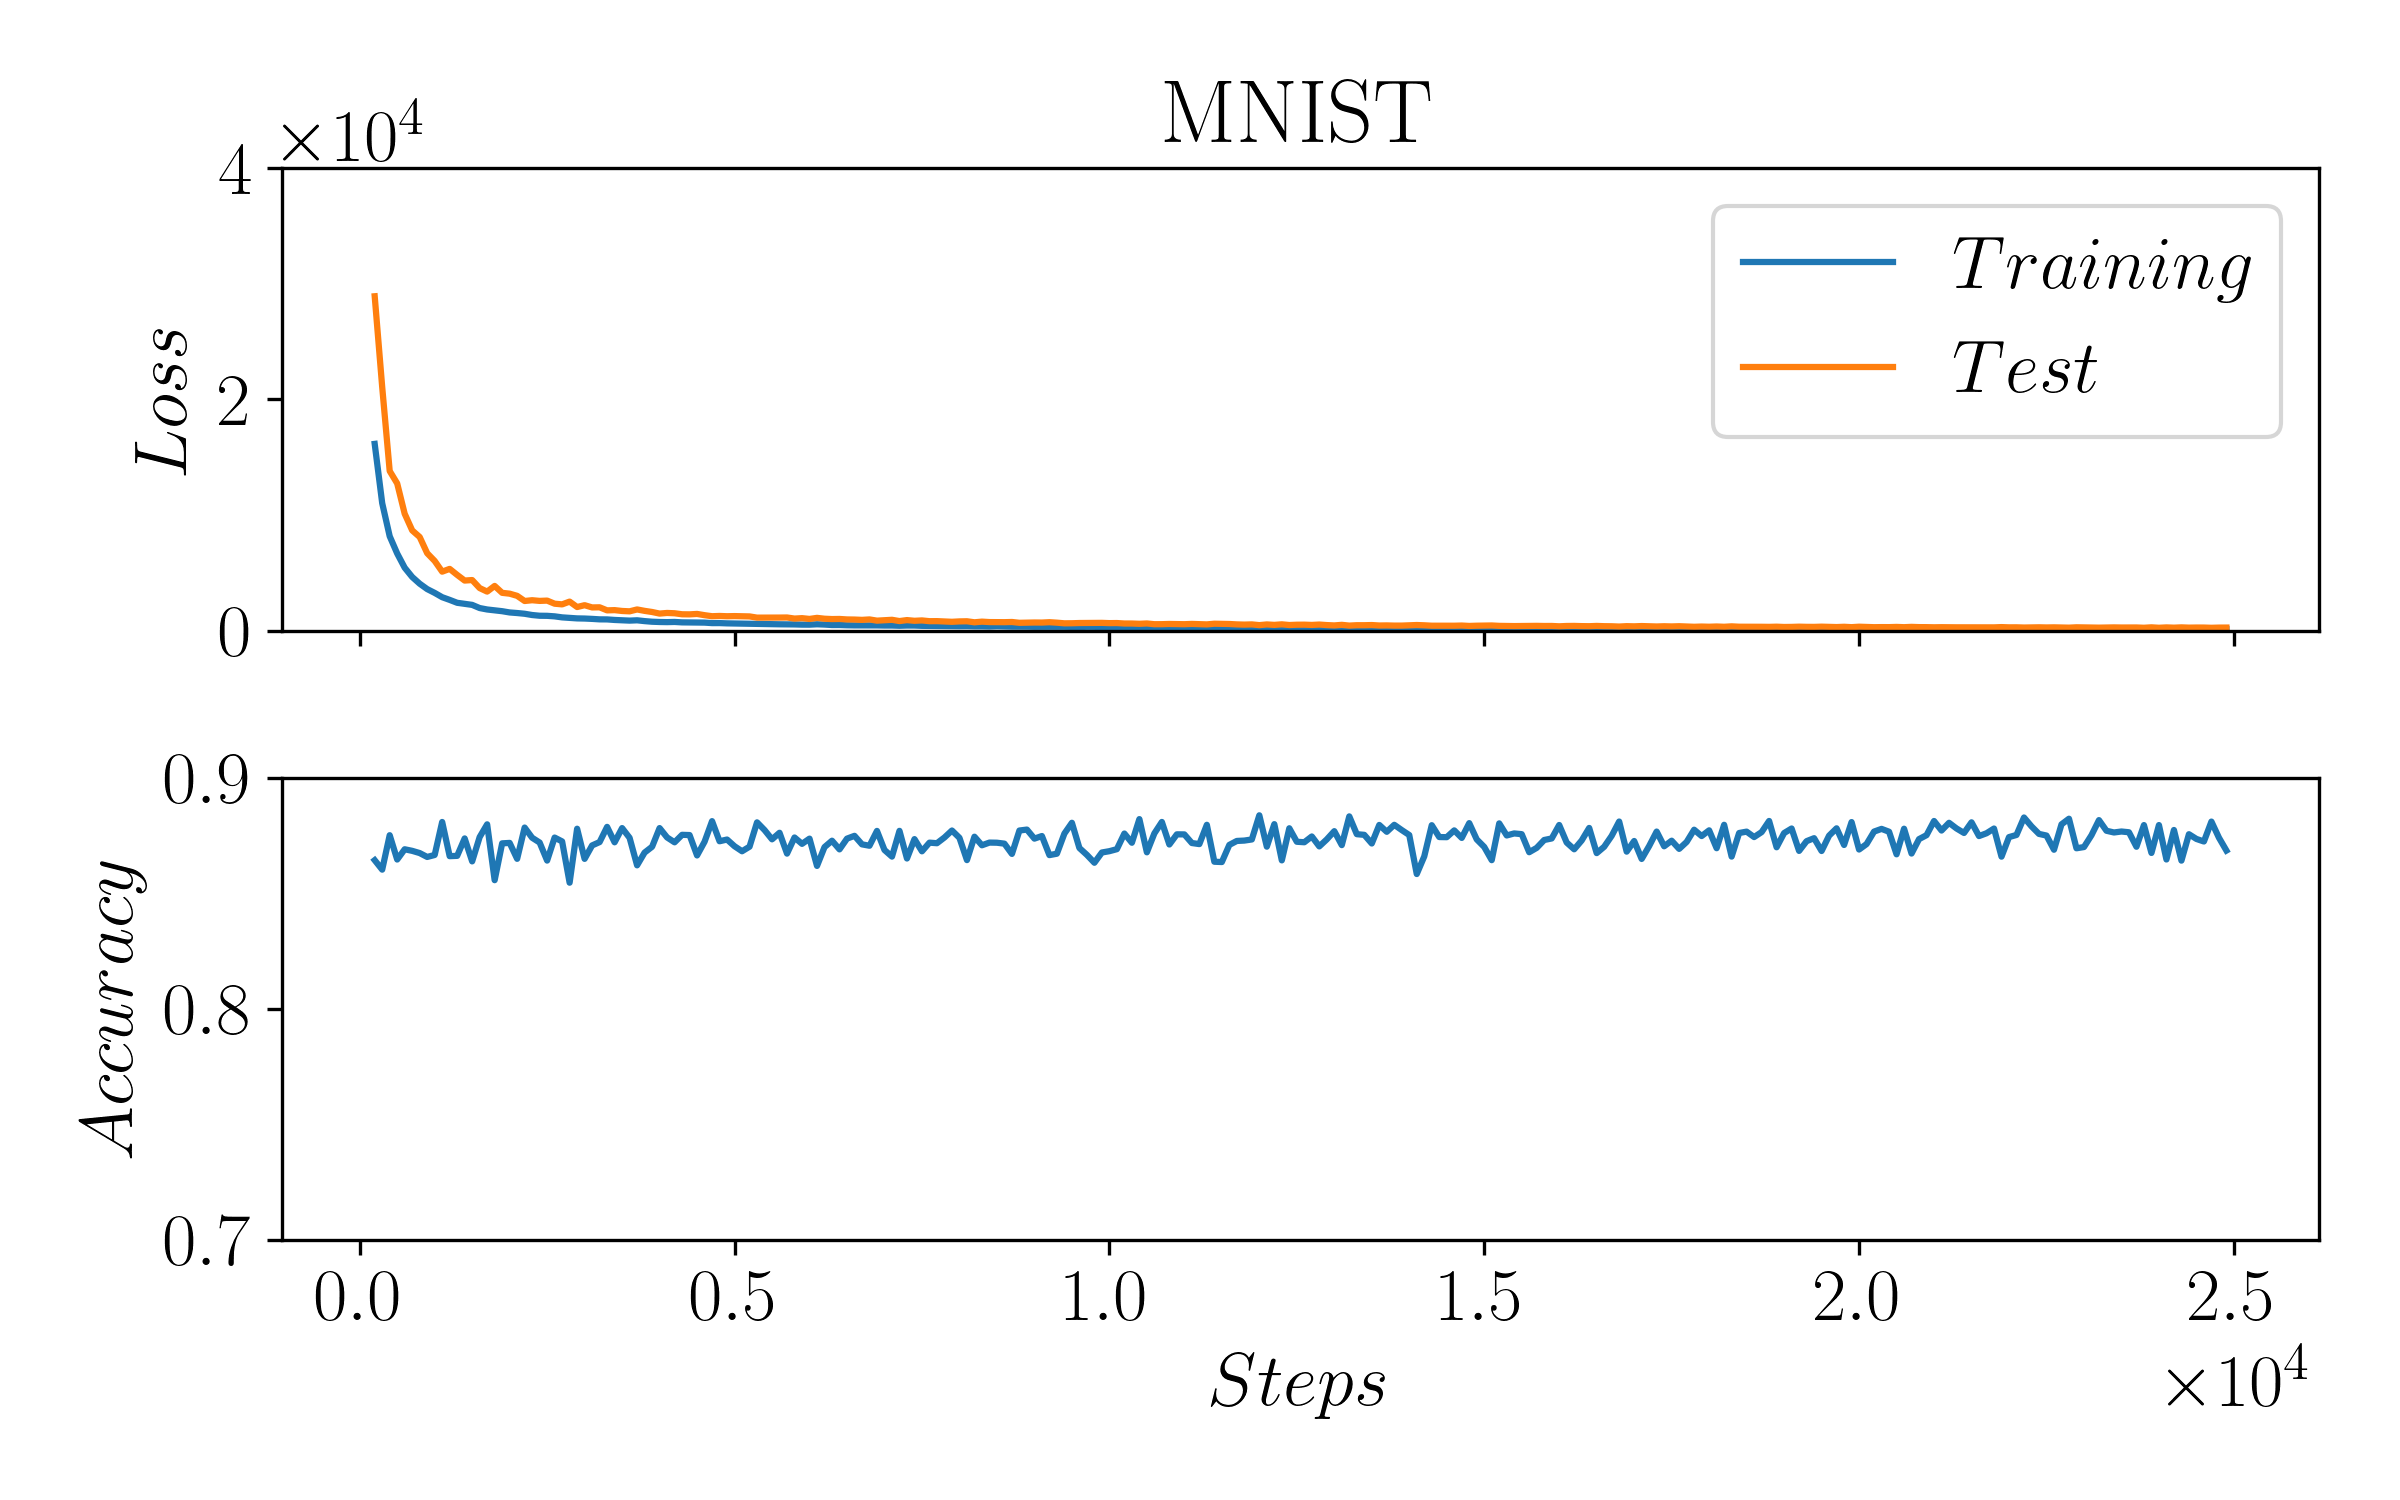
\includegraphics[width=12cm]{assets/ml_metrics.png}
    \caption{Support Vector Machine training loss, test loss and accuracy averaged over 10 runs on MNIST dataset}
    \label{figure:mlmetrics}
\end{figure}

Compute metrics mean training step time and cpu utilization percentage had variability but did not clearly decrease or increase during model training. \improvement{add figure} Memory use steadily grew in a stepwise manner over time during model training. \improvement{add figure} \improvement{add details}

\improvement{add shape of different algorithms and datasets}

\subsection{Effects of hyperparameter changes on system metrics}

Batch size

Learning rate

alpha


\begin{figure}[h]
    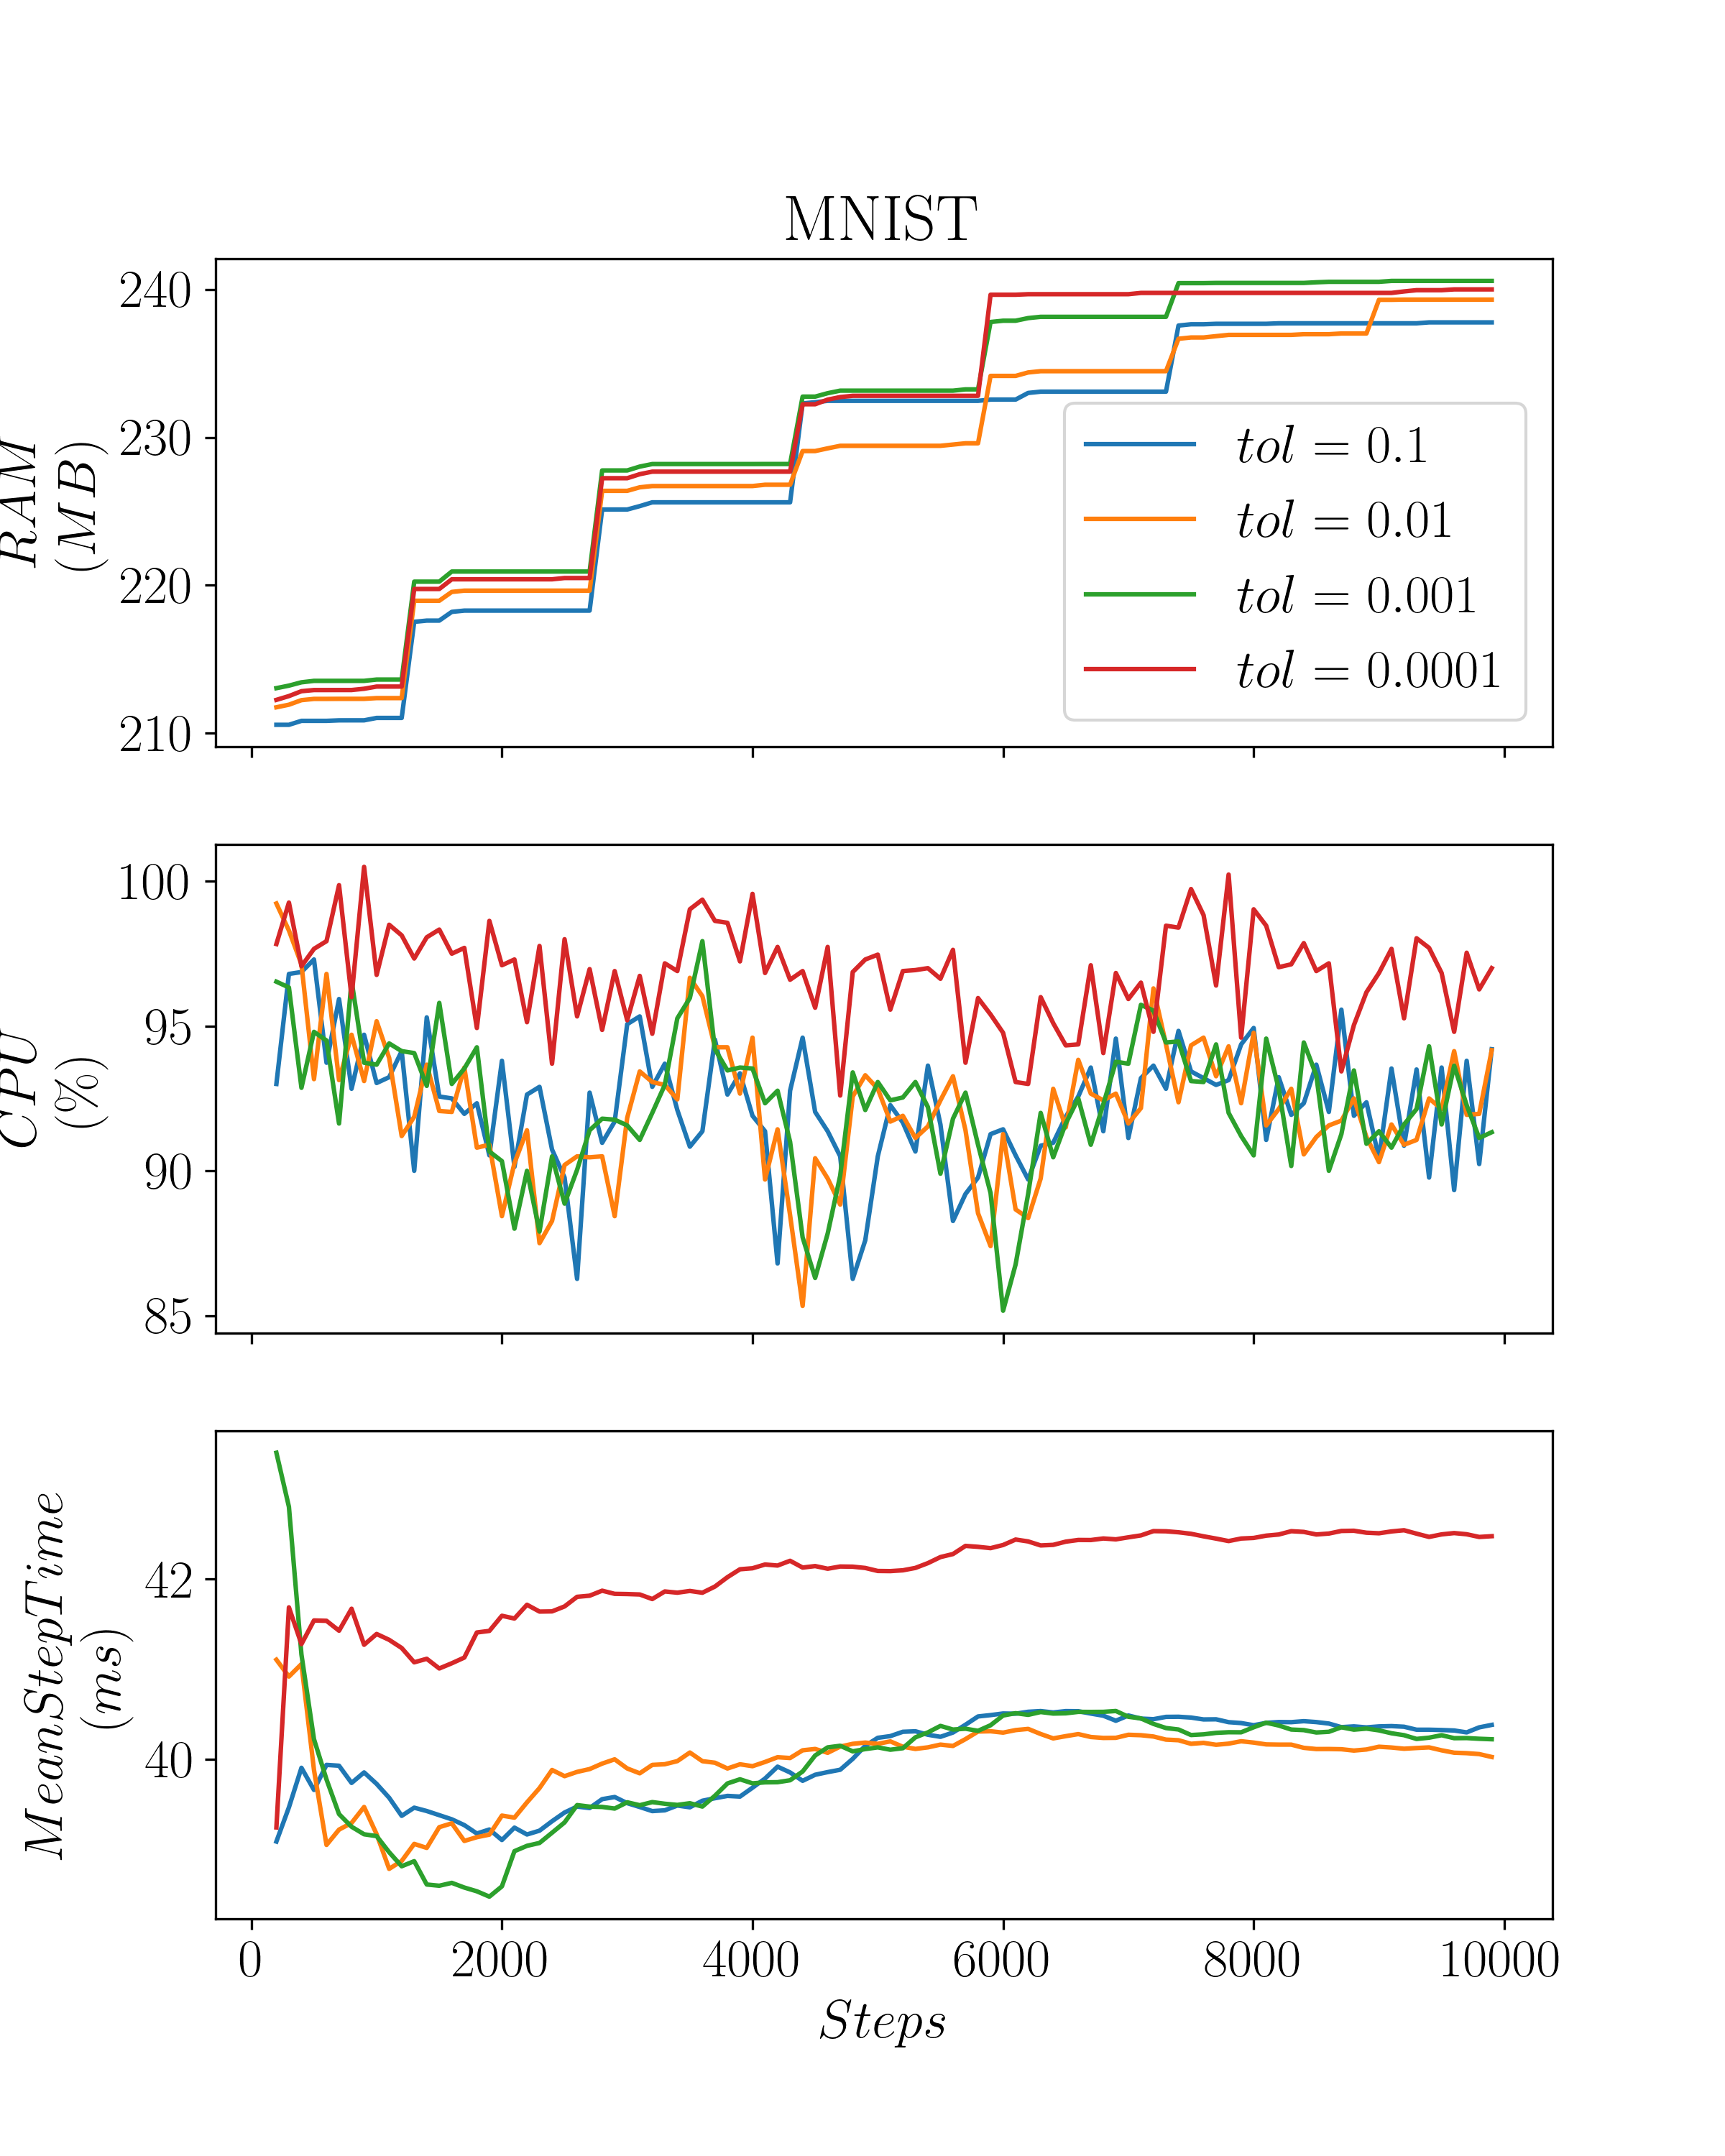
\includegraphics[width=12cm]{assets/tol.png}
    \caption{TODO placeholder image: Effect of tol hyperparameter on system performance metrics}
    \label{figure:tol}
\end{figure}

\subsection{Effects of early stopping on computational budgets}



\improvement[inline]{ML performance threshold}
\improvement[inline]{ram threshold}

